% --------------------------------------------------------------
% This is all preamble stuff that you don't have to worry about.
% Head down to where it says "Start here"
% --------------------------------------------------------------
 
\documentclass[12pt]{article}
 
\usepackage[margin=1in]{geometry} 
\usepackage{multicol,caption}
\usepackage{graphicx}
\usepackage{multicol}
\usepackage{lipsum}
\usepackage{float}
\usepackage{graphics}
\usepackage[utf8x]{inputenc}

\newcommand{\N}{\mathbb{N}}
\newcommand{\Z}{\mathbb{Z}}
 \newenvironment{Figure}
  {\par\medskip\noindent\minipage{\linewidth}}
  {\endminipage\par\medskip}

\begin{document}

 
\title{Progetto Sistemi Intelligenti - Alberto Borghese
Riconoscitore di cifre manoscritte}%replace X with the appropriate number
\author{Francesco Bertolotti} %if necessary, replace with your course title
 
\maketitle
 
\section{Introduzione}
Come concordato, ho deciso di sfruttare alcuni concetti mostrati
durante il corso, per implementare un riconoscitore di caratteri manoscritti, 
sfruttando le reti neurali. Il progetto è stato svolto in python utilizzando diverse librerie.
E' stato utilizzato il dataset del MNIST.


\section{Dipendenze}
Le librerie utilizzate in python sono elencate di seguito:
\begin{enumerate}
    \item Keras\cite{keras}: Una nota API ad alto livello per reti neurali.
    \item numpy: Un pacchetto per il calcolo scientifico.
    \item optparse: Un pacchetto per la gestione di opzioni CLI.
    \item tensorflow\cite{tensorflow}: engine backend per keras, capace di sfruttare anche le GPU.
    \item opencv\cite{opencv}: API per la gestione di immagini.
\end{enumerate}

\section{Modelli}
Per costruire un riconoscitore efficace sono stati testati diversi modelli:
\begin{enumerate}
    \item MLPNN: Una rete a diversi livelli completamente conessa.
    \item CNN\cite{cnn}: Una rete convoluzionale che sfrutta kernel di dimensioni ridotte
               per la classificazione delle immagini.
    \item Committees: Comitati di esperti che prendono decisioni basate sulla maggioranza.
\end{enumerate}


\begin{multicols}{2}
    Di seguito il modello di rete convuluzionale utilizzato per il riconoscitore.\\\\

    \bigskip
    \noindent
    \begin{minipage}{\linewidth}
        \centering
        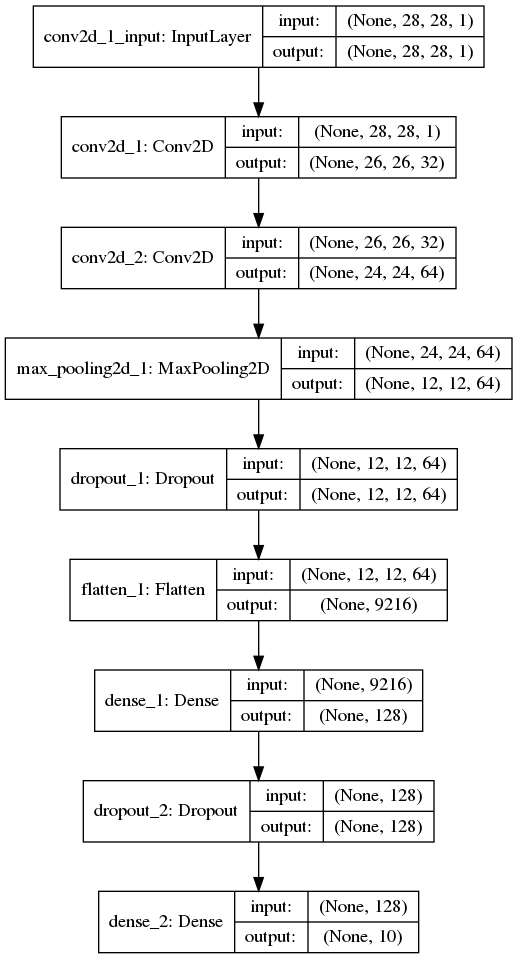
\includegraphics[width=6cm]{../mnist_models/CNN2D_type0-batch128/model.png}
        \captionof{figure}{Struttura della rete convulozionale}\label{fig:cc}
    \end{minipage}
    \bigskip

    Vengono utilizzati 32 e successivamente 64 filtri convoluzionali di dimensione 3x3.
    A questo punto viene applicato un filtro di max pooling per ridurre ulteriormente
    la dimensionalità (9216 output), in ultimo applichiamo
    un MLPNN completamente connesso, con un singolo hidden layer di 128 neuroni,
     per distinguere le classi. Inoltre è stato utilizzato
    un dropout di 0.2 sui singoli pesi.\\\\Mostriamo la figura relativa a uno dei 
    modelli MLPNN utilizzati (ne sono stati provati diversi).

    \bigskip
    \noindent
    \begin{minipage}{\linewidth}
        \centering
        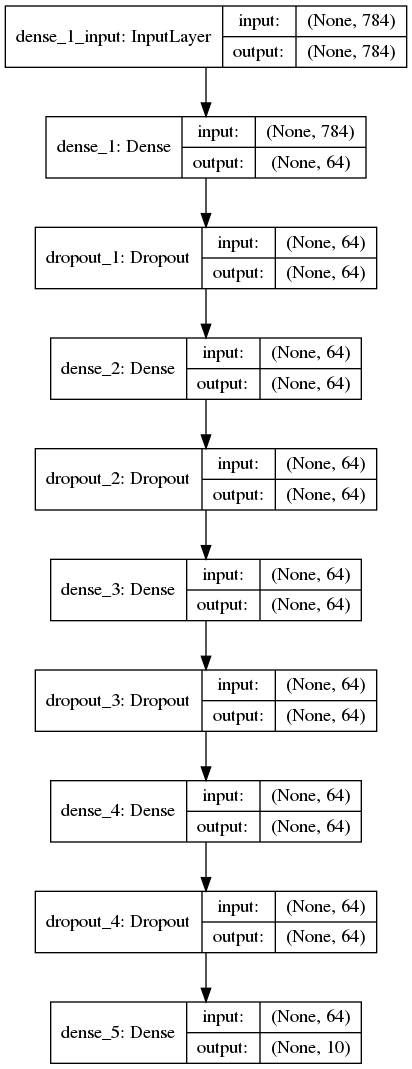
\includegraphics[width=6cm]{../mnist_models/MLPNN_type1-batch128-balanced/model.png}
        \captionof{figure}{Struttura della rete neurale}\label{fig:cc}
    \end{minipage}
    \bigskip

    In questo caso, ho utilizzato 5 layer ciascuno da 64 neuroni più l'uliltimo da 10. 
    Anche questa volta con un dropout di 0.2.\\


    Per entrambi i modelli l'output è rappresentato da un vettore di 10 elementi
    di valore compreso tra 0 e 1, di cui solo il massimo è rappresentante della
    classe associata.\\

\end{multicols}

    Come funzione di attivazione è sempre stata utilizzata la RELU per i layer nascosti
    e la SoftMax per i layer di output, per avere una interpretazione probabilistica
    sugli output della rete.

\section{Trainig and Testing}

Il dataset utilizzato è quello classico del mnist e anche come partizionamento
tra train e test set è stato utilizzato quello proposto dal dataset originale.\\
Per quanto riguarda l'addestramento è stato utilizzato il classico algoritmo
di discesa del gradiente \cite{gradient}, in particolare è stato utilizzata una variante detta 
rmsprop\cite{rmsprop} che va a mediare il nuovo aggiornamento (dei pesi) con quelli passati, in modo
tale da avere una discesa più regolare.\\
Come Loss function ad ogni iterazione si ha 0 se la classe proposta dalla rete
è corretta 1 altrimenti.\\
La dimensione dei batch utilizzata è solitamente 128, ma mi sono preso la libertà di
provare con dimensioni differenti: 1, 128, 512, 1024 e full.\\
Lo script trainer.py si occupa per l'appunto di effettuare l'addestramento della
rete neurale, e al lancio di quest'ultimo è possibile inserire diverse opzioni da linea
di comando.

\begin{enumerate}
    \item "-d", "--directory": permette di scegliere una cartella di destinazione
    per il salvataggio del modello.
    \item "-s", "--batch": permette di scegliere la dimensione del batch con cui
    effettuare l'addestramento.
    \item "-e", "--epochs": permette di scegliere il numero di epoche per
    cui si vuole fare l'addestramento.
    \item "-b", "--balance": permette di specificare se si vuole effettuare
    un bilanciamento delle diversi classi prima di cominciare l'addestramento
    \item "-c", "--committee": permette di selezionare il numero di reti che si 
    vogliono addestrare, con lo scopo di generare una pool di esperti che prenderà
    le decisioni per maggioranza.
    \item "-m", "--modelname": permette di scegliere il tipo del modello, questi
    sono descritti nel file "models.py"
\end{enumerate}
Ad ogni addestramento verrano generati i seguenti file:

\begin{enumerate}
    \item "test\_loss\_acc.png", "train\_loss\_acc.png": sono il plot dell'accuratezza e della loss
    rispetto al training set e al test set generato epoca per epoca.
    \item "model.png": l'immagine rappresentante il modello.
    \item "model0.best.hdf5": il mogliore modello addestrato in termini di accuratezza e loss.
\end{enumerate}

Di seguito l'andamento di loss e accuracy per quanto riguarda la reti:

\begin{figure}[H]{}
    \centering
    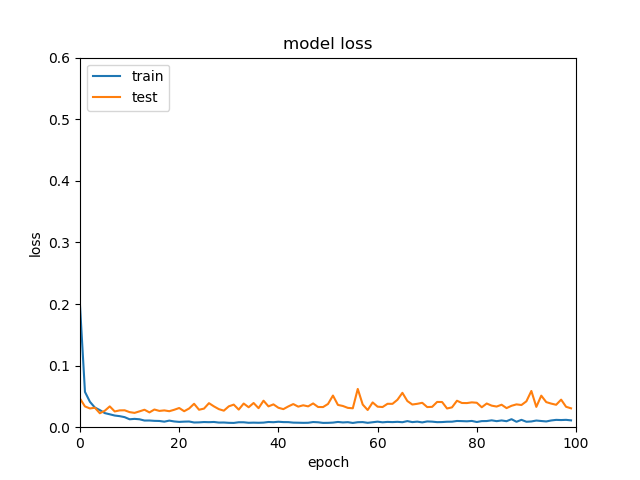
\includegraphics[scale=0.8]{../mnist_models/CNN2D_type0-batch128-balanced/0test_loss_acc.png}
    \captionof{figure}{loss della rete convoluzionale}\label{fig:cc}
\end{figure}

\begin{figure}[H]{}
    \centering
    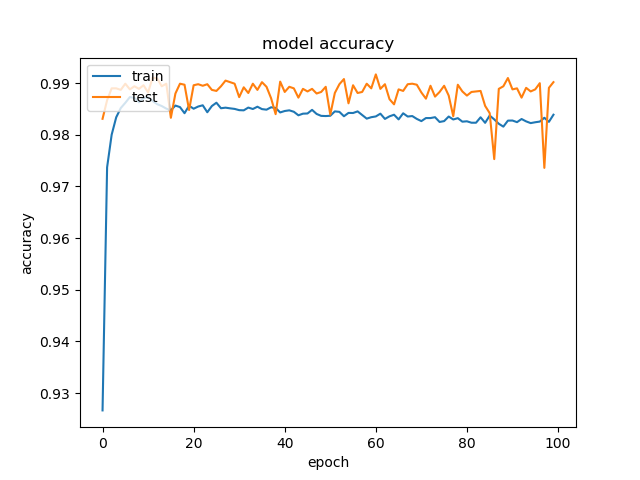
\includegraphics[scale=0.8]{../mnist_models/CNN2D_type0-batch128-balanced/0train_loss_acc.png}
    \captionof{figure}{accuracy della rete convoluzionale}\label{fig:cc}
\end{figure}

\begin{figure}[H]{}
    \centering
    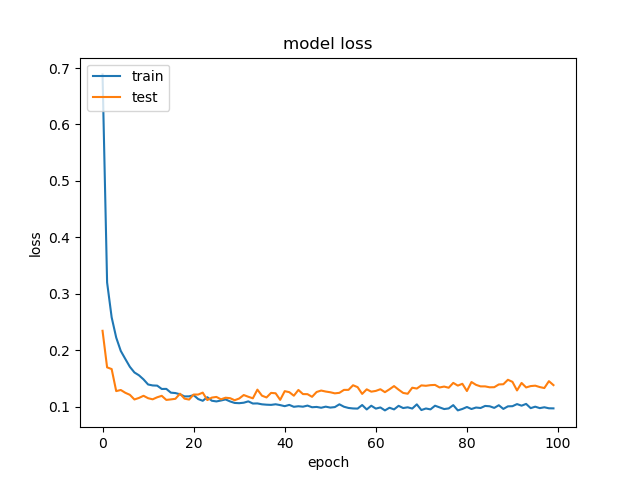
\includegraphics[scale=0.8]{../mnist_models/MLPNN_type1-batch128-balanced/0test_loss_acc.png}
    \captionof{figure}{loss del percetrone multilivello}\label{fig:cc}
\end{figure}

\begin{figure}[H]{}
    \centering
    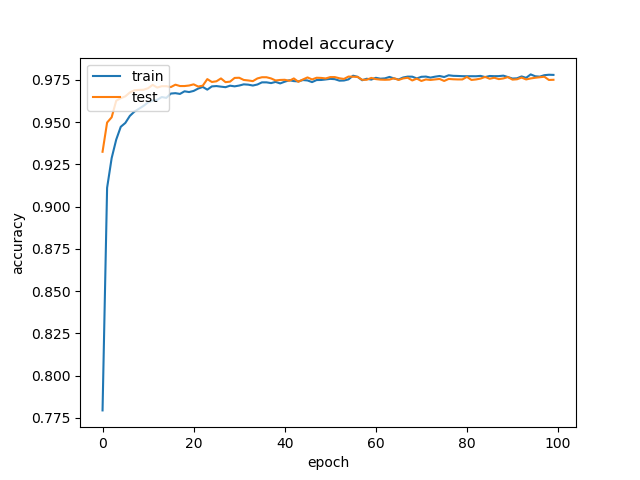
\includegraphics[scale=0.8]{../mnist_models/MLPNN_type1-batch128-balanced/0train_loss_acc.png}
    \captionof{figure}{accuracy del percetrone multilivello}\label{fig:cc}
\end{figure}


\section{Using}

Una volta addestrato il modello viene utilizzato dallo script recognizer.py
che carica inizialmente uno o più reti e poi le sfrutta per riconoscere le cifre disegnate su 
di una finistra aperta tramite opencv\cite{opencv}.
Alcuni esempi sono dati nelle immagini segueti:


\begin{figure}[H]{}
    \centering
    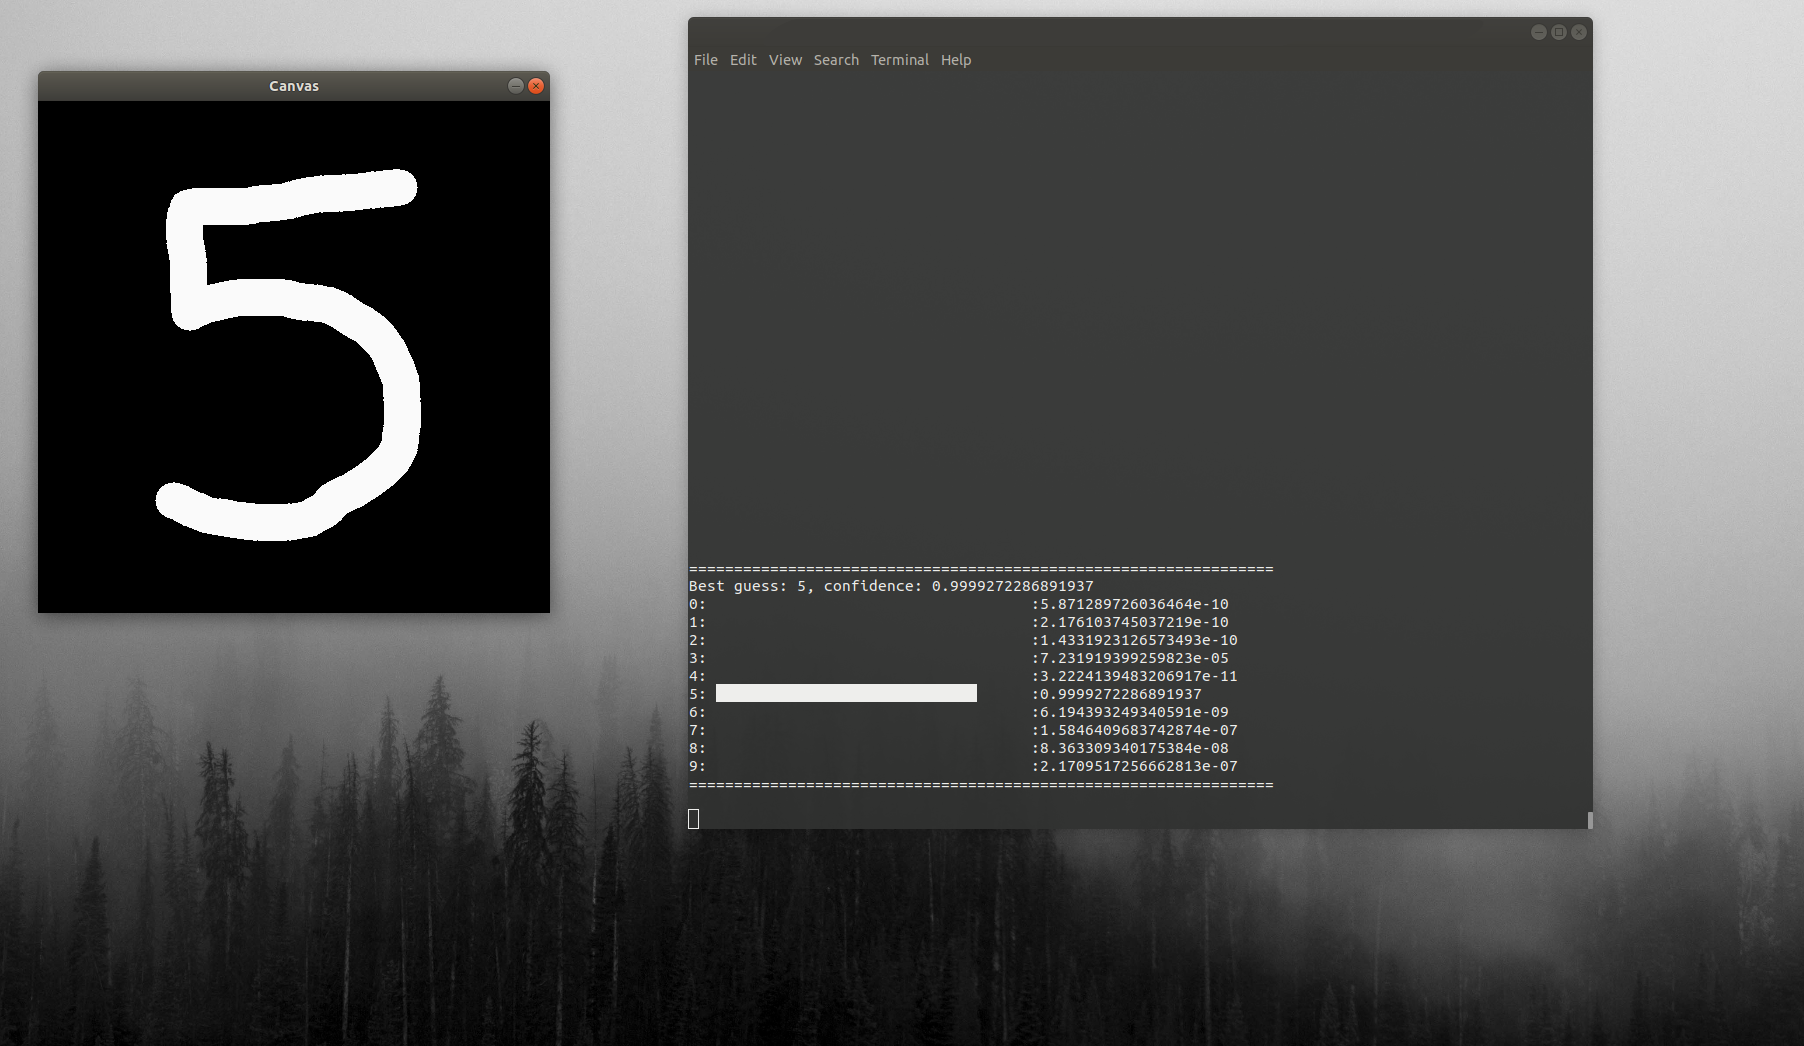
\includegraphics[scale=0.25]{../images/1.png}
\end{figure}

\begin{figure}[H]{}
    \centering
    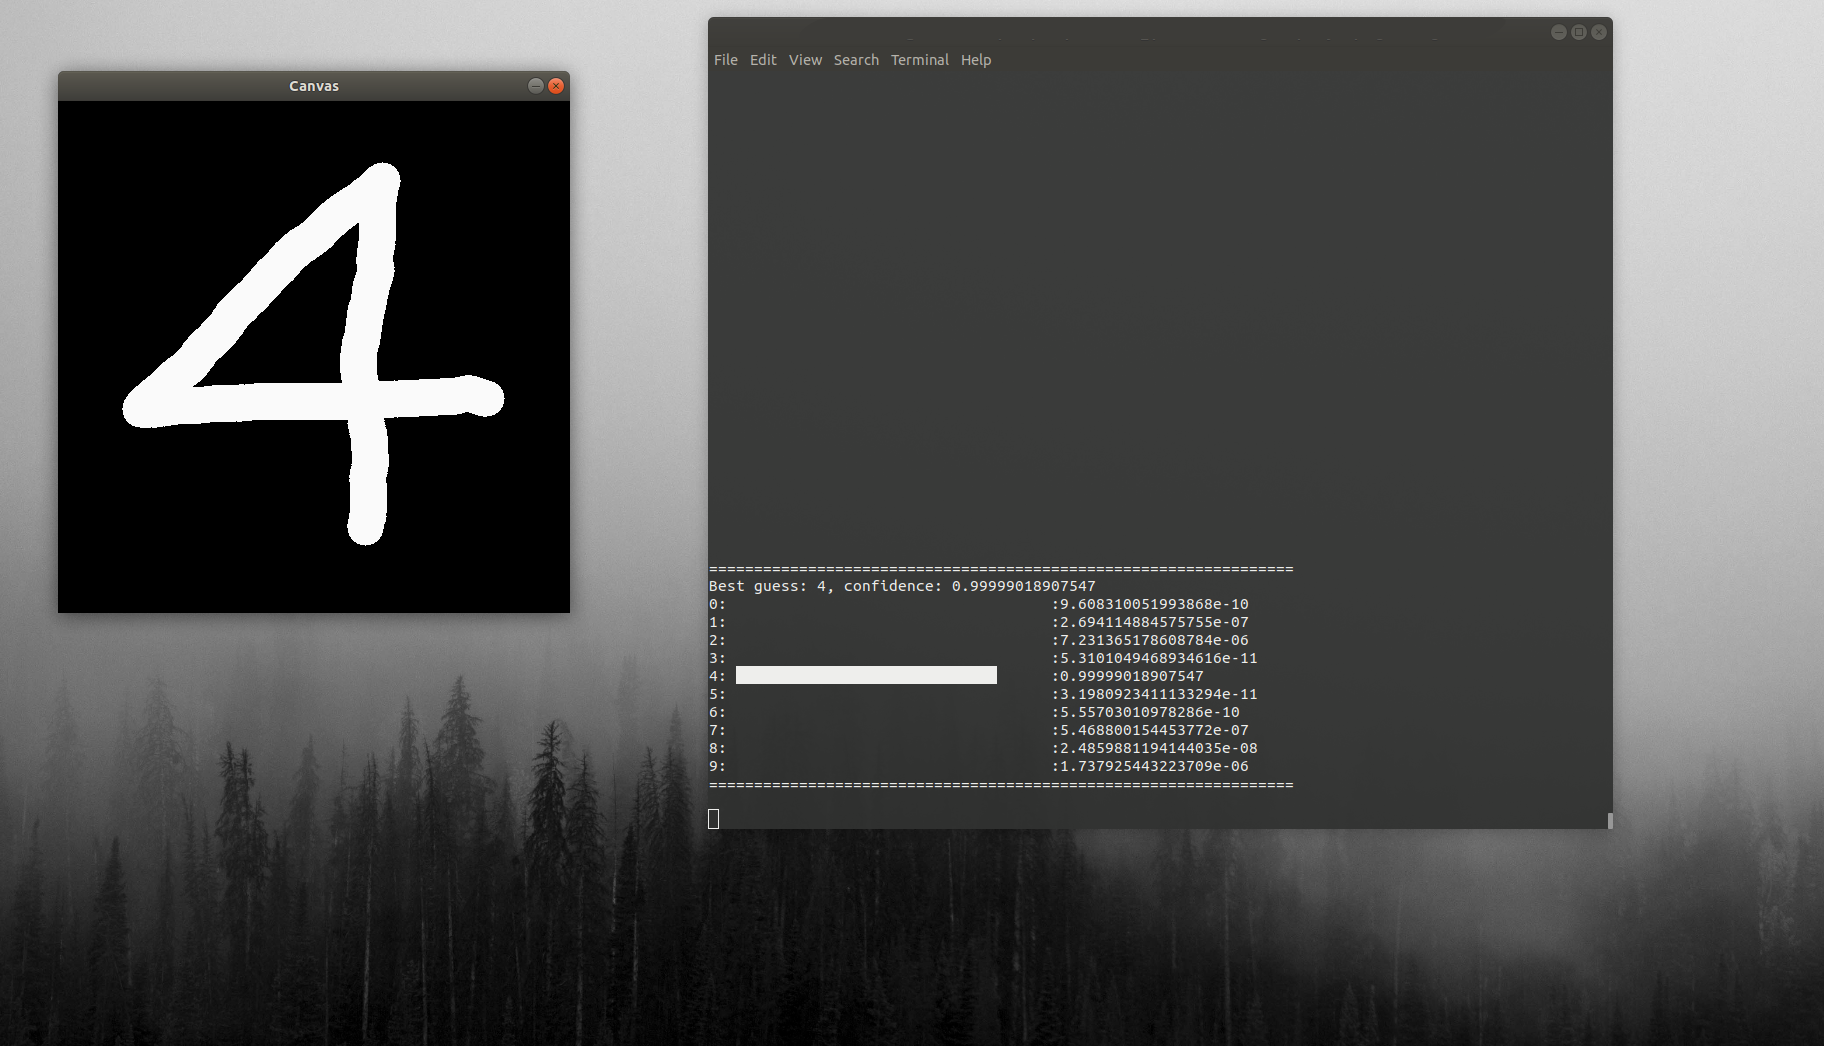
\includegraphics[scale=0.25]{../images/2.png}
\end{figure}

\begin{figure}[H]{}
    \centering
    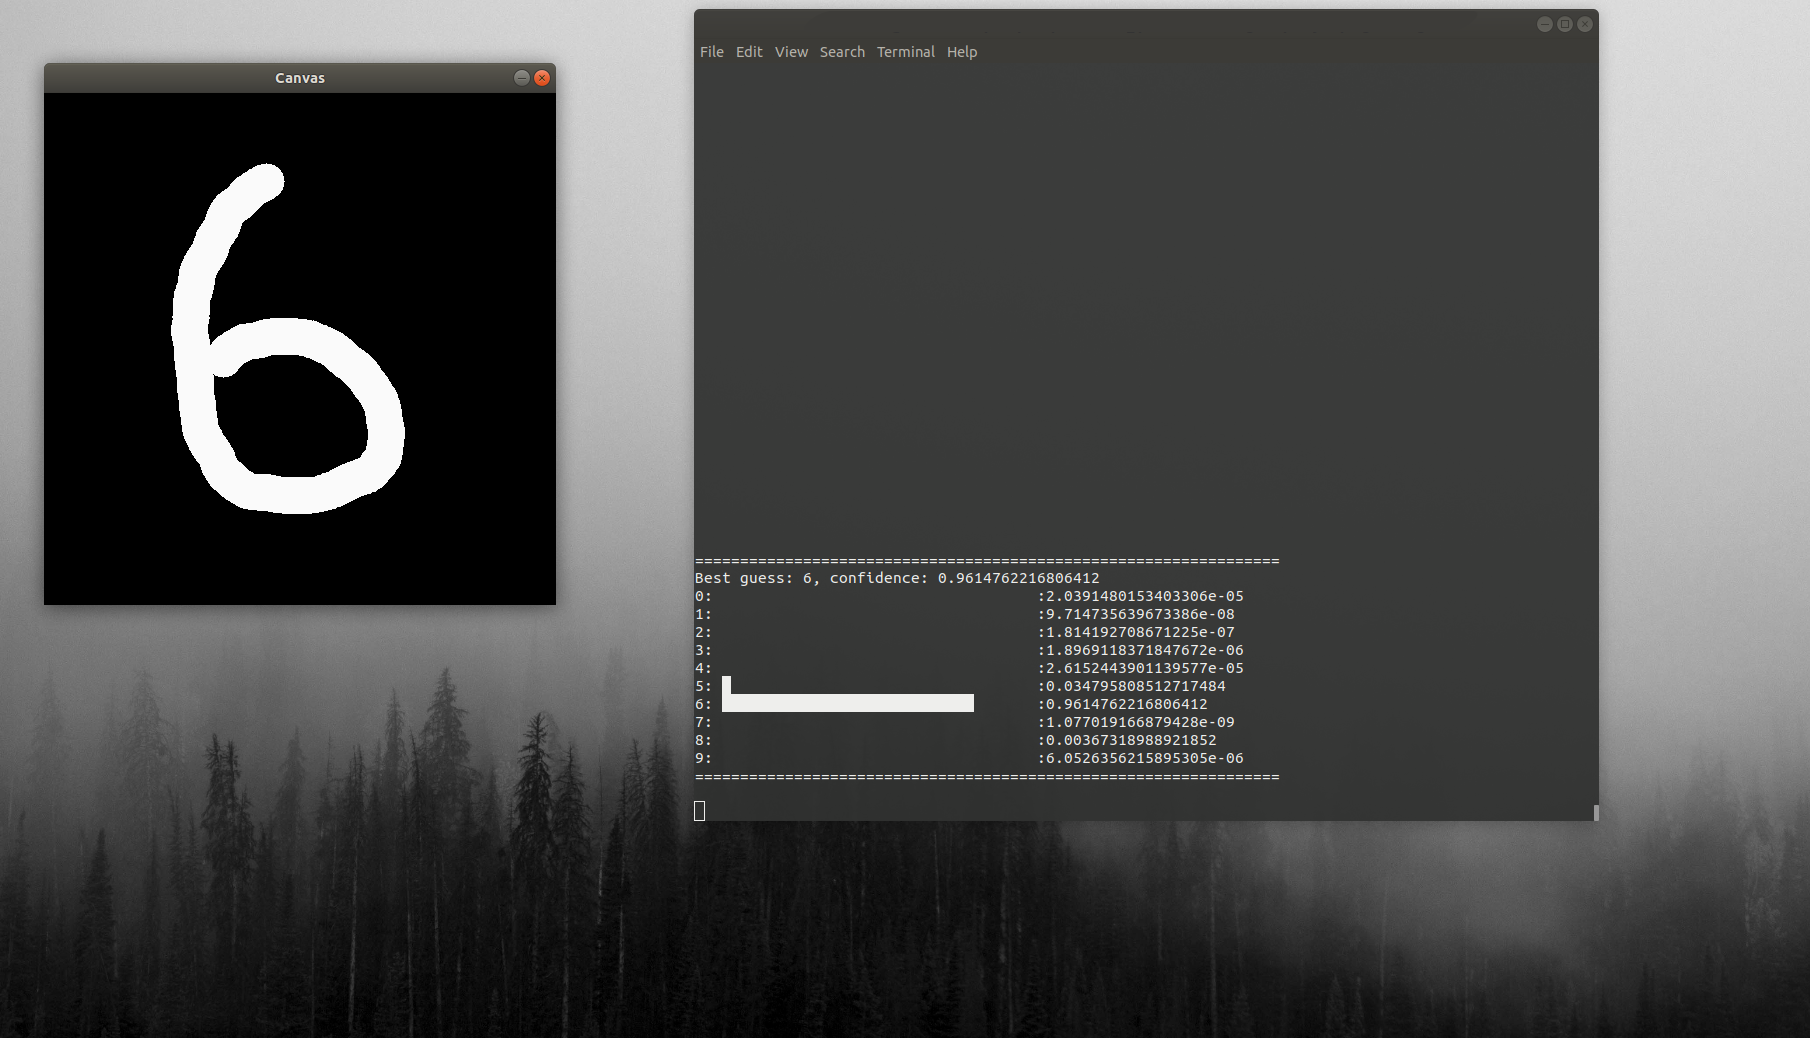
\includegraphics[scale=0.25]{../images/3.png}
\end{figure}

\begin{figure}[H]{}
    \centering
    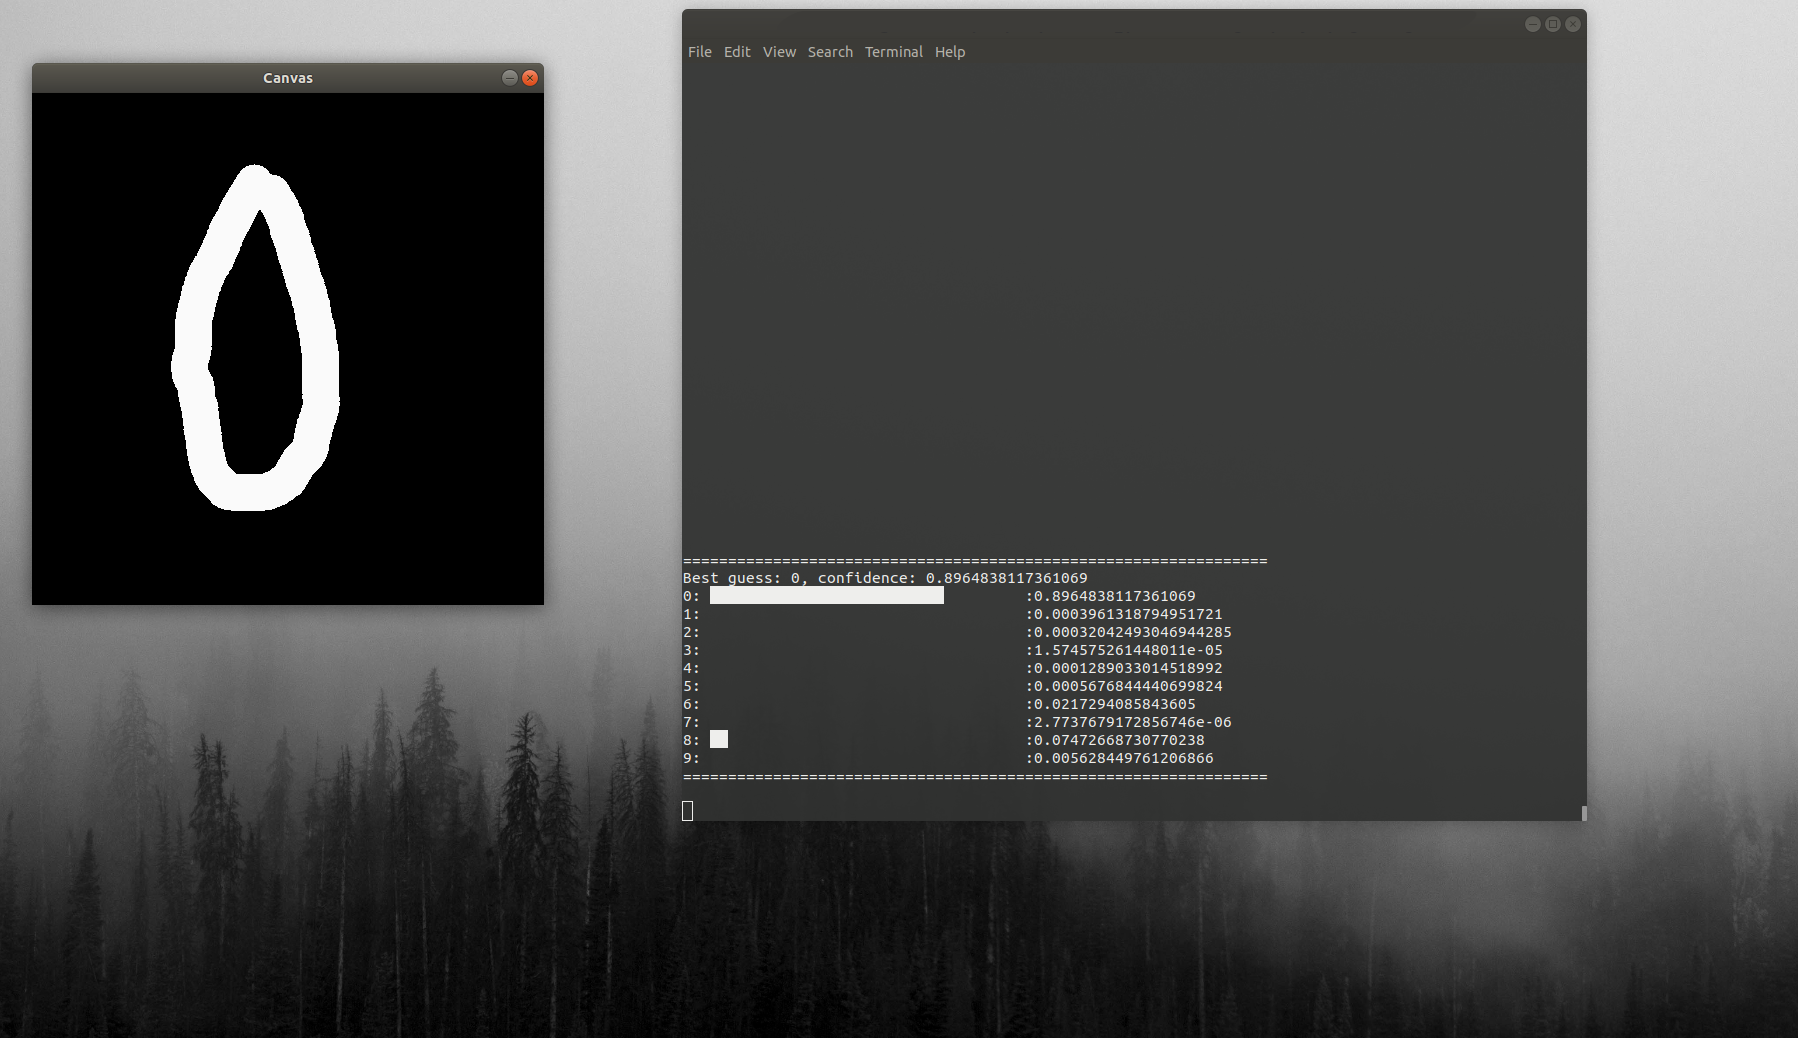
\includegraphics[scale=0.25]{../images/4.png}
\end{figure}

\begin{figure}[H]{}
    \centering
    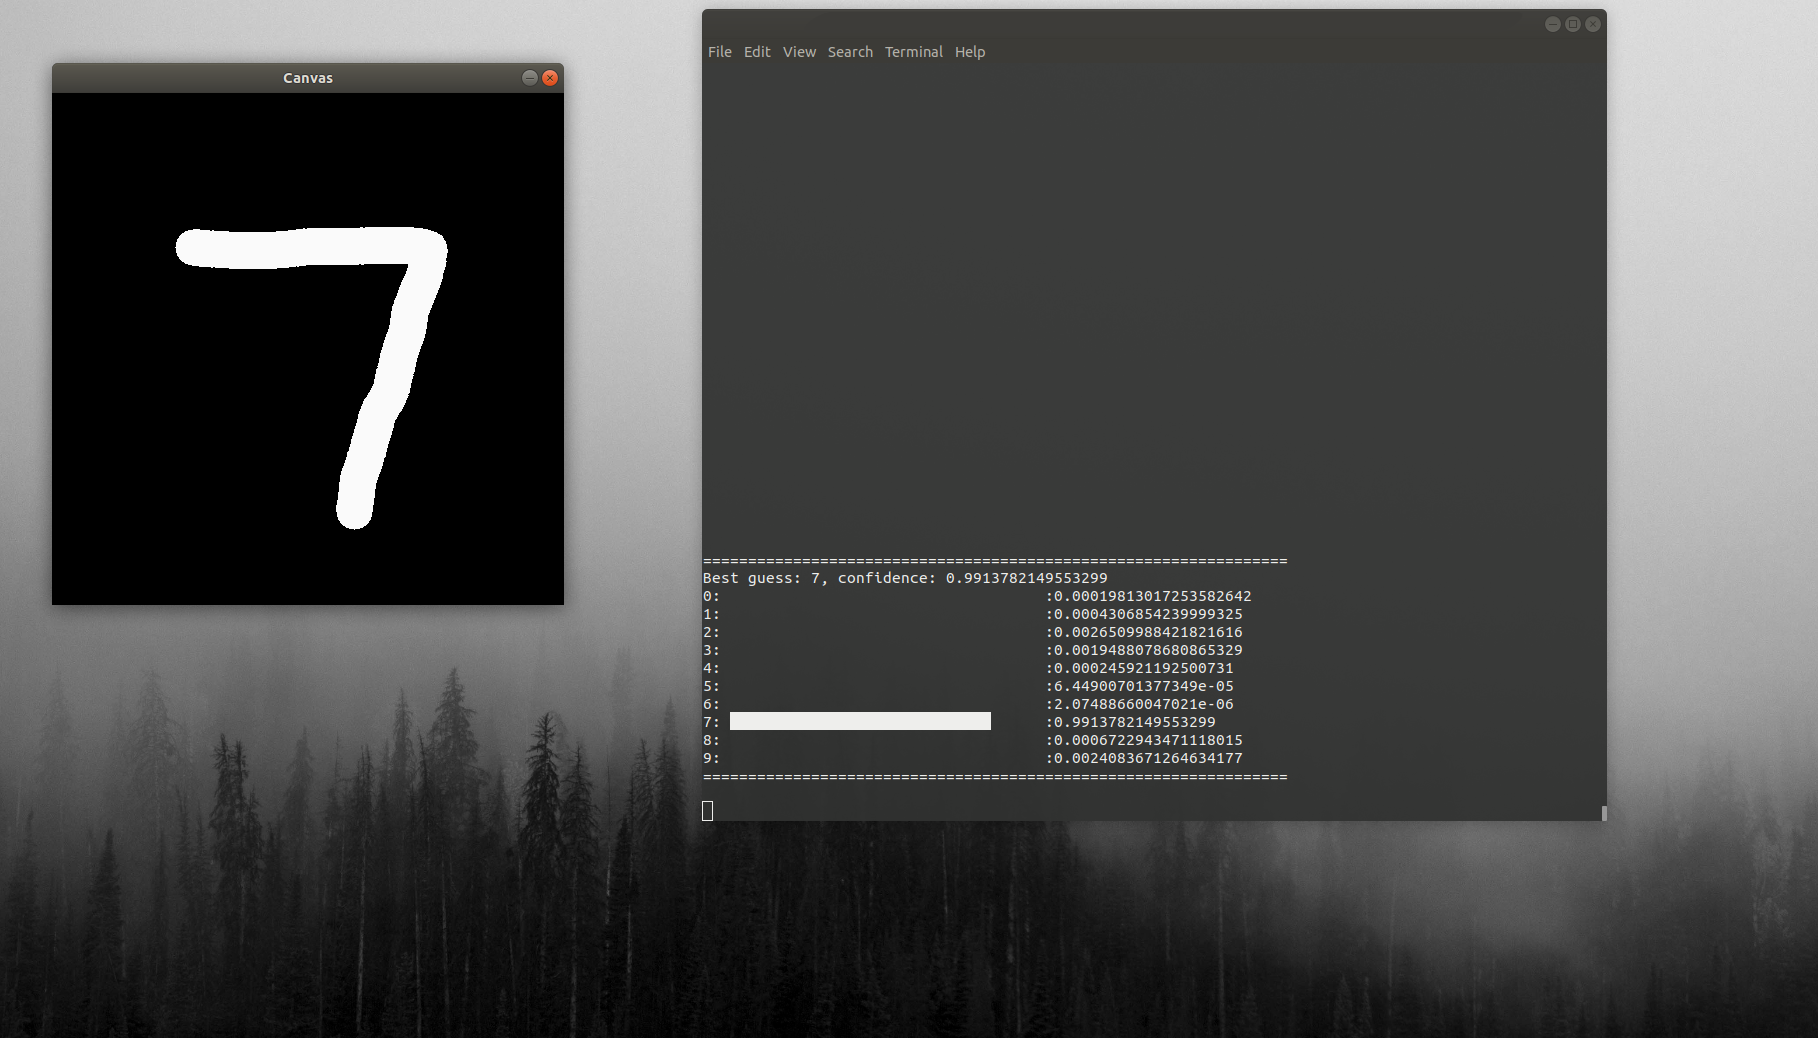
\includegraphics[scale=0.25]{../images/5.png}
\end{figure}

\begin{figure}[H]{}
    \centering
    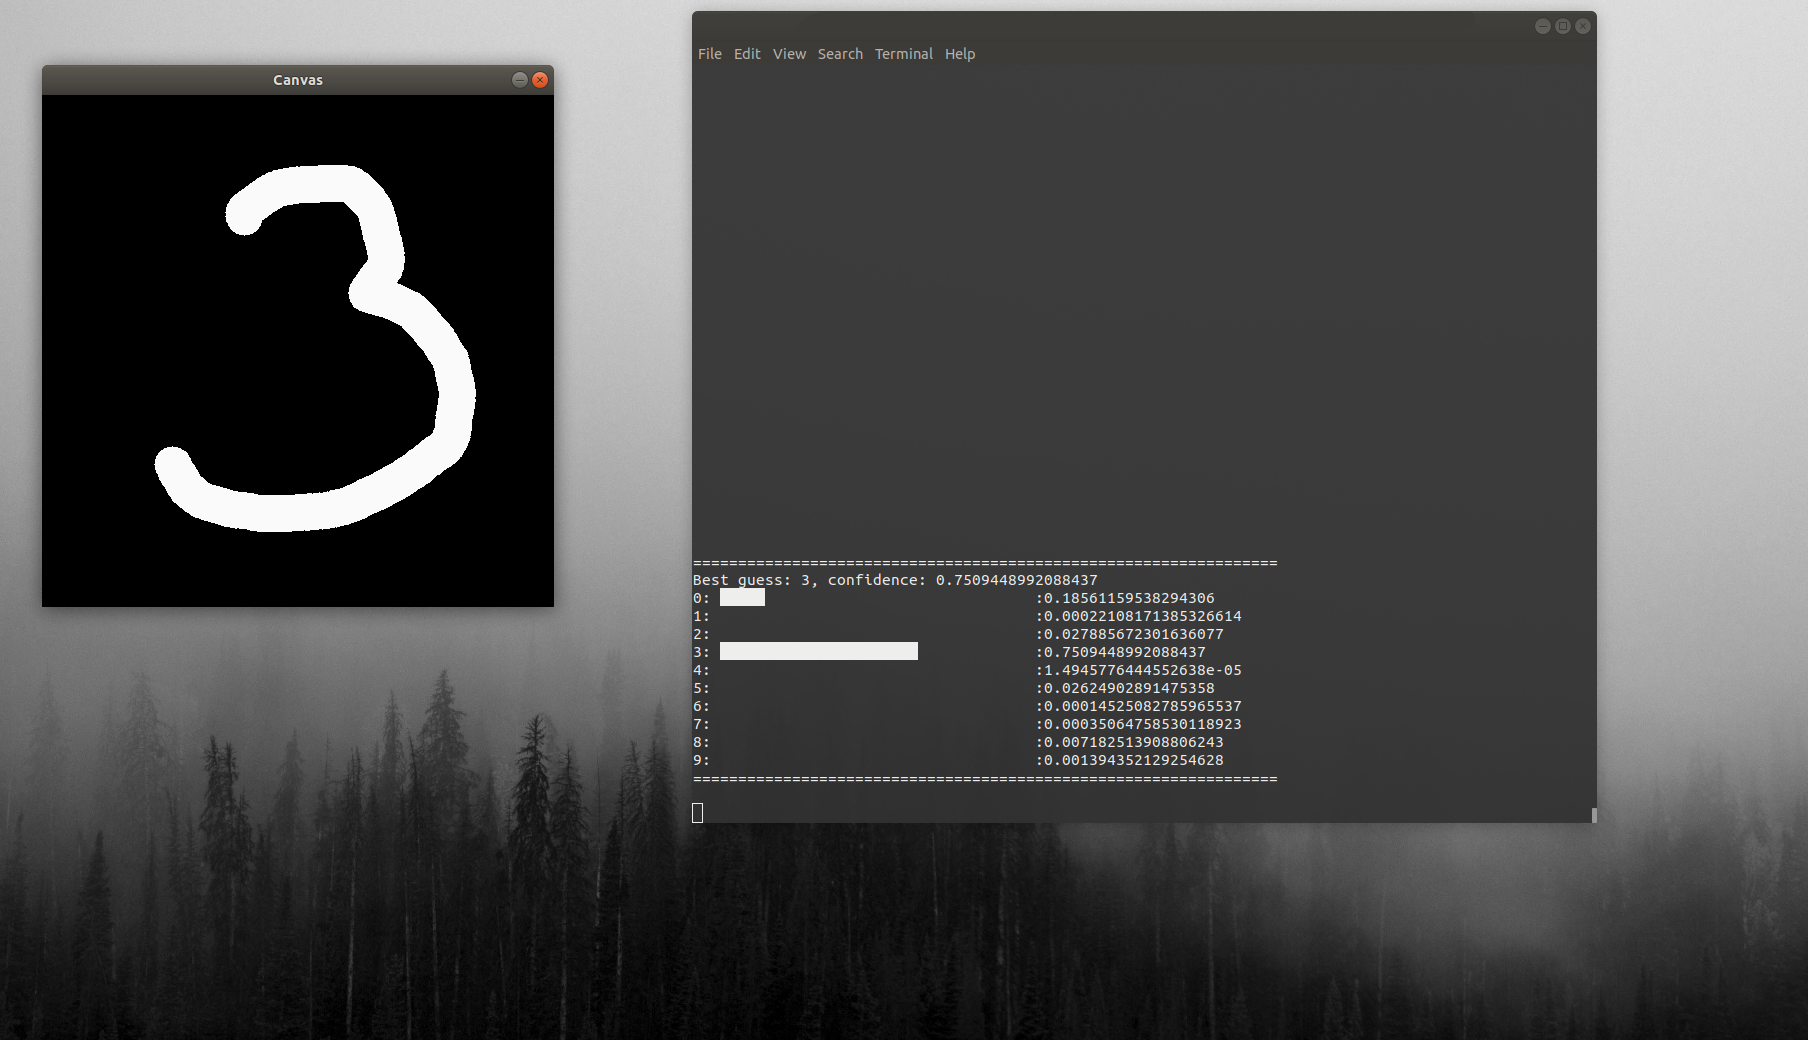
\includegraphics[scale=0.25]{../images/6.png}
\end{figure}

In questo caso il programma utilizzava un comitato di 20 reti convoluzionali
per prendere le decisioni.

\section{Conclusions}

In conclusione abbiamo che la reti convoluzionali si comportano meglio 
rispetto al percettrone multilivello in termini di accuratezza loss e
tempi di training necessari.
Il riconoscitore funziona complessivamente bene, anche se in certi casi
commette errori, soprattutto quando le cifre sono simili tra di loro (es. 5,6 o 2,7).
Sicuramente è possibile avere un riconoscitore più preciso andando
ad ampliare il dataset con casi più diversificati e più numerosi, 
o eventualmente, facendo un oversampling delle immagini più critiche. 

\section{References}

\begin{thebibliography}{9}

\bibitem{gradient}
  Claude Lemarcéchal,\\
  \textit{https://www.math.uni-bielefeld.de/documenta/vol-ismp/40\_lemarechal-claude.pdf},
  2010.

\bibitem{rmsprop}
   Geoffrey E. Hinton,\\
  \textit{http://www.cs.toronto.edu/~tijmen/csc321/slides/lecture\_slides\_lec6.pdf}.

\bibitem{cnn}
   Alex Krizhevsky, Ilya Sutskever, Geoffrey E. Hinton, 
   ImageNet Classification with Deep Convolutional Neural Networks,
  \textit{https://papers.nips.cc/paper/4824-imagenet-classification-with-deep-convolutional-neural-networks.pdf}.

\bibitem{keras}
   \textit{https://github.com/keras-team/keras}

\bibitem{tensorflow}
   \textit{https://www.tensorflow.org/}

\bibitem{opencv}
   \textit{https://opencv.org/}

\end{thebibliography}

\end{document}
